\section{Assembler Directives \& Addressing Modes}

\subsection{Directives}

\begin{tabular}{lp{0.3\textwidth}}
    \textbf{Directive} & \textbf{Description} \\
    $\mathbf{SECTION}$ & \textit{Defines the beginning of a relocatable section} \\
    $\mathbf{EQU}$     & \textit{Assigns an expression to a name. Not redefinable} \\
    $\mathbf{DC}$      & \textit{Defines one or more constants and their names. Will be stored at the set location} \\
    $\mathbf{DS}$      & \textit{Allocates memory(RAM) for variables} \\
\end{tabular}

\textit{
    The Assembler-Directive $\mathbf{SECTION}$ defines program- and
    data section. Those section can be moved freely within the memory (relocative
    assembling), \textbf{after} the \textbf{assembly} process is finished. \\
    The final memory area location happens after the linking process. The locations
    of those sections can therefor be defined in the \textbf{Linker-Parameterfile}.
}

\subsection{Basic Assembler Program}

\begin{lstlisting}
; include definitions
include 'MC9S08JM60.inc'

; -- globals
GLOBAL _Startup ; define start of programm
GLOBAL main
GLOBAL dummy    ; Dummy Interrupt Service Routine

; -- equations
StackSize: EQU   $60   ; stack size
pi:        EQU   31416 ; example of random equ

; -- stack
DATA_STACK: SECTION
TofStack:  DS    StackSize-1 ; definiton of "Top of Stack"
BofStack:  DS    1           ; definition of "Bottom of Stack"

; -- create space for data
DATA:   SECTION
var1:   DS    1   ; Example of a 1 Byte Variable
Array1: DS    $20 ; Example of an Array of $20 Bytes

; -- setup constants
CONST:     SECTION
Maske1:      DC.B    %00000001
Parameter1:  DC.B    $3A    ; DC with a point
Parameter2:  DC.W    57100  ; word with int value
Reserve_Par: DS      16     ; reserve empty 16 Bytes
VarArray:    DS.W    3      ; reserve 3 Words
STRING1:     DC.B    10,"Hello",$0D

; -- program start (initialisation)
PROGRAMM:   SECTION ; Code Segment
_Startup:           ; Resetvektor points to this
Stackinit:  LDHX  #(BofStack+1)
            TXS          ; decrement TXS, thats why +1 BofStack
            LDA   #$00
            STA   SOPT1  ; Disable Watchdog

; -- actual program
main:
    ; turn on backligths of the car
    BSET    PTDD_PTDD2, PTDD
    BSET    PTDDD_PTDDD2, PTDDD

    CLR     RamLoc

    BCLR    PTGDD_PTGDD0, PTGDD
    BCLR    PTGDD_PTGDD1, PTGDD
    BCLR    PTGDD_PTGDD2, PTGDD
EndlessLoop:
    ; load joystick values
    MOV     RamLoc, PTGD
    JMP     EndlessLoop

; (=ensure program end if endlessloop is missing)
EndLoop:    BRA     *

; catch any unexpected interrupts
dummy:          BGND
                BRA     dummy

\end{lstlisting}

\subsection{Addressing Modes}

\begin{itemize}
    \item{\textit{\textbf{Immediate}: 1 Byte operand in instruction (LDA \#\$01)}}
    \item{\textit{\textbf{Inherent}: no operand required (e.g. NOP, INCA..)}}
    \item{\textit{\textbf{Direct}: onlu direct page, 1 address Byte}}
    \item{\textit{\textbf{Extended}: whole 64k area, 2 address Bytes}}
    \item{\textit{\textbf{Indexed}: with SP (Stack pointer) or HX (7 sub modes)}}
    \item{\textit{\textbf{Relative}: for branches, PC=PC+2+two's compl.}}
\end{itemize}

\textit{
    Different addressing modes of the same instruction type use differnet
    operation codes (e.g. LDA-MM: A6; LDA-DIR: B6). \\
}

\subsubsection{Immediate (IMM)}

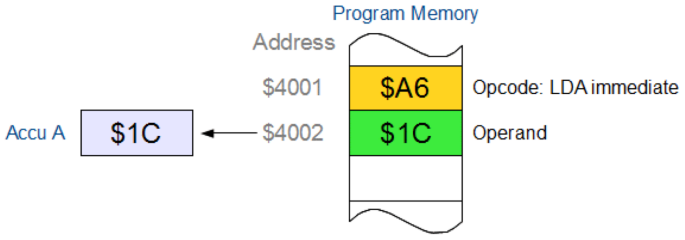
\includegraphics[width=0.5\textwidth]{addressmode-immediate.png}

\textit{
    \textbf{Immediat adressing} mode: the following Byte of the operation code
    is immediately used as the operand. \\
    Example: \textbf{LDA \#\$1C}
}

\subsubsection{Inherent (INH)}

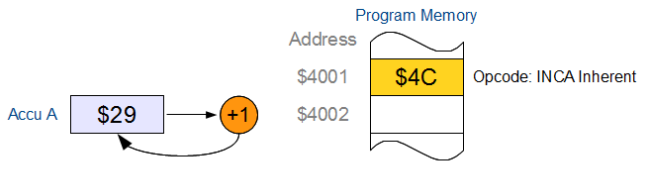
\includegraphics[width=0.5\textwidth]{addressmode-inherent.png}

\textit{
    \textbf{Inherent addressing} mode: no explicit operand address needed.
    All operands are in the CPU-registers \\
    Example: \textbf{INCA}
}

\subsubsection{Direct (DIR)}

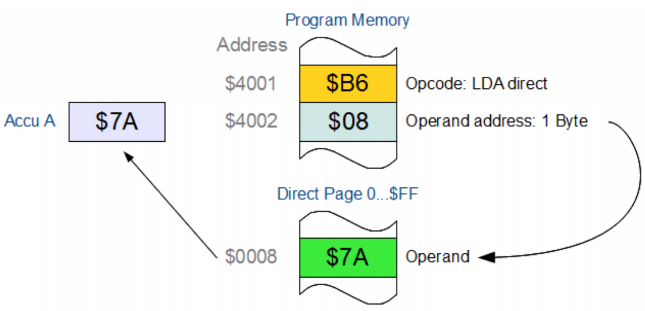
\includegraphics[width=0.5\textwidth]{addressmode-direct.png}

\textit{
    \textbf{Direct addressing} mode: After the operation code, the
    \textbf{1-Byte} operand address follows in the program memory. \\
    Only operands in the address section between \$00 and \$FF are
    supported. (The Direct Page Registers 0x00-0xAF, Direct Page RAM 0xB0-0xFF) \\
    Example: \textbf{LDA \$08}
}

\subsubsection{Extended (EXT)}

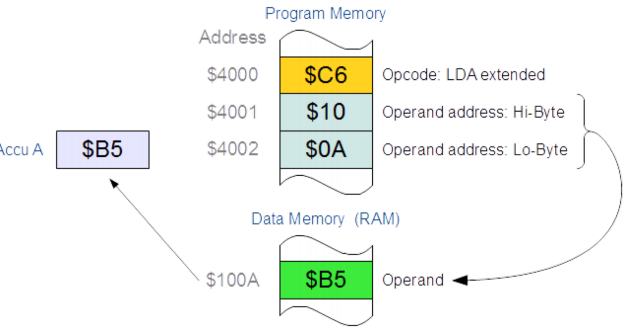
\includegraphics[width=0.5\textwidth]{addressmode-extended.png}

\textit{
    \textbf{Extended addressing} mode: After the operation code, the \textbf{2-Byte}
    operand address follows in the program memory. \\
    Supports the whole address section between 0x0000 - 0xFFFF. But is also slower. \\
    Example: \textbf{LDA \$34,X}
}

\subsubsection{Indexed (IX1)}

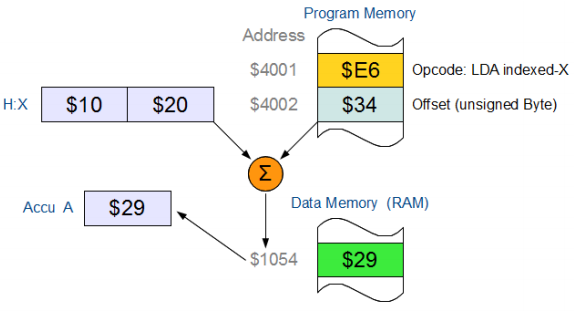
\includegraphics[width=0.5\textwidth]{addressmode-indexed.png}

\textit{
    \textbf{Indexed addressing} mode: uses the \textbf{HX} or \textbf{SP} register. \\
    Through indexed addressing the final assigned operand address is dependent from
    the program behaviour (address arithmetics).
}

\textit{Following are sub modes of the indexed addressing mode}

\begin{tabular}{lp{0.25\textwidth}l}
    $\mathbf{IX}$   & \textit{Indexed addressing with H:X, without offset}
                    & \scriptsize{\textbf{LDA  X}} \\
    $\mathbf{IX1}$  & \textit{Indexed addressing with H:X and \textbf{8-bit offset}}
                    & \scriptsize{\textbf{LDA  \$34, X}} \\
    $\mathbf{IX2}$  & \textit{Indexed addressing with H:X and \textbf{16-bit offset}}
                    & \scriptsize{\textbf{LDA  \$34A5, X}} \\
    $\mathbf{IX+}$  & \textit{
                            Indexed addressing with \textbf{H:X} and \textbf{H:X
                            Increment}. Only for MOV and CBEQ
                            (Compare Accu with value on the address that
                            is stored in the H:X register. If values are
                            equal, jump to Label and increment H:X)
                            instructions
                        }
                    & \scriptsize{\textbf{CBEQ  X+, Label}} \\
    $\mathbf{IX1+}$ & \textit{Same as IX+, with \textbf{Increment} and \textbf{8-bit offset} (Only available for instruction CBEQ)}
                    & \scriptsize{\textbf{CBEQ  \$34,X+, Label}} \\
    $\mathbf{SP1}$  & \textit{Same as IX1, but with Stackpointer SP instead of H:X.}
                    & \scriptsize{\textbf{LDA  \$34, SP}} \\
    $\mathbf{SP2}$  & \textit{Same as IX2, but with Stackpointer SP instead of H:X.}
                    & \scriptsize{\textbf{LDA  \$34A5, SP}} \\
\end{tabular}

\subsubsection{Relative (REL)}

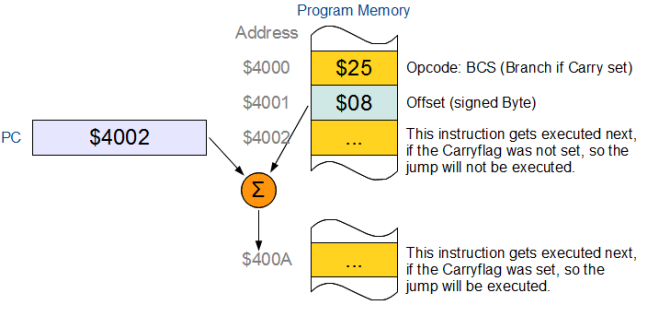
\includegraphics[width=0.5\textwidth]{addressmode-relative.png}

\textit{
    \textbf{PC relative addressing} mode: is only used with BRANCH-Instructions. \\
    The following Byte after the operand is a \textbf{two's complement} offset
    to the already increased program counter. \\
    The address range with relaive addressing is -126 to +129. 129, since
    the PC is incremented before and after the jump (+2).
}
